\documentclass[12pt]{report}

\usepackage{mathtools}
\usepackage{amsmath}
\usepackage{systeme}
\usepackage{siunitx}
\usepackage[T1]{fontenc}
\usepackage{hyperref}
\usepackage{bigfoot}
\usepackage[numbered, framed]{matlab-prettifier}
\usepackage{filecontents}
\usepackage{graphicx}
\hypersetup{
colorlinks,
citecolor=black,
filecolor=black,
linkcolor=black,
urlcolor=black
linkto=all,
}

\newenvironment{simplechar}{%
   \catcode`\^=12
}{}

\title{Numerical Methods, project A, Number 31}
\author{Krzysztof Rudnicki\\ Student number: 307585 \\ Advisor: dr Adam Krzemieniowski}
\date{\today}

\let\ph\mlplaceholder % shorter macro
\lstMakeShortInline"

\lstset{
  style              = Matlab-editor,
  basicstyle         = \mlttfamily,
  escapechar         = ",
  mlshowsectionrules = true,
}

\begin{document}


\maketitle
\tableofcontents

\chapter{Problem 1 - Finding machine epsilion}

\section{Problem}
Write a program finding macheps in the MATLAB environment
\section{Theoretical Introduction}
\subsection{Definition of machine epsilion}
Machine epsilion is the maximal possible relative error of the floating-point representation. (Tatjewski, p.14)
Machine epsilion is equal to $2^{-t}$ where t is number of bits in the mantissa.
In our case when We use IEEE Standard 754, mantissa is 53 bits long with first bit omitted as it is always equal to '1', so We technicaly work with 52 bits mantissa which makes the machine epsilion equal to: $2^{-52} = 2.220446\mathrm{e}{-16}$

\subsection{Practical applications of machine epsilion}
Since macheps is connected to IEEE754 standard it is always equal to the same number, which means that we can safely compare results from different machines without worrying about their individual errors. Before standards, everyone could use any way of representing floats.

Macheps is also essential when We calculate cumulation of errors of given mathematical operation.

\newpage
\section{Solution}

\subsection{Matlab code}
\begin{lstlisting}
macheps = 1;
while 1.0 + macheps / 2 > 1.0
    macheps = macheps/2;
end
\end{lstlisting}
Code above shifts macheps one bit to the right each iteration (by dividing by 2), it ends when We run out of mantissa bits which renders us unable to save smaller number. Due to underflow the value of macheps becomes 0 and therefore 1.0 > (macheps / 2) > 1.0 will become false.

\section{Discussion of the result}
\begin{simplechar}
\begin{lstlisting}
format long
disp("Display calculated macheps:")
disp(macheps);
disp("Display actual eps:")
disp(eps);
disp("Display 2^-52")
disp(2^-52)
disp("Display difference between calculated macheps and actual eps:")
disp(macheps - eps)
disp("Display difference between 2^-52 and actual eps:")
disp(2^-52 - eps) \
disp("Display difference between calculated macheps and 2^-52:")
disp(macheps - 2^-52)
\end{lstlisting}
\end{simplechar}
Display calculated macheps:
     \[2.220446049250313\mathrm{e}{-16}\]

Display actual eps:
     \[2.220446049250313\mathrm{e}{-16}\]

Display $2^{-52}$:
     \[2.220446049250313\mathrm{e}{-16}\]

Display difference between calculated macheps and actual eps:
     \[0\]

Display difference between $2^{-52}$ and actual eps:
          \[0\]

Display difference between calculated macheps and $2^{-52}$:
         \[0\]

As expected they are all equal to eachother. It means that our method of calculating macheps was correct.

\chapter{Problem 2 - Solving a system of n linear equations - indicated method}

\section{Problem}
Write a program solving a system of \textit{n} linear equations Ax = b using the indicated method (Gaussian elimination with partial pivoting).

\section{Theoretical Introduction}
Gaussian elimination with partial pivoting consists of 3 main steps:
\subsection{Transform matrix into upper-triangular matrix}

\subsubsection{Starting conditions}
We start with the system of linear equations looking like this:

\[
\begin{matrix}

&a_{11}x_1 &{}+&a_{12}x_2&+&\dots&+&a_{1n}x_n &=&b_1,\\

&a_{21}x_1 &{}+&a_{22}x_2&+&\dots&+&a_{2n}x_n &=&b_2,\\

&\vdots    &&\vdots      & &     & &  \vdots  & &\vdots\\

&a_{n1}x_1&{}+&a_{n2}x_2&+&\dots &+&a_{nn}x_n&=&b_n.

\end{matrix}
\]

In order for this method to work all the elements of "diagonal" line:
\[ a_{11}, a_{22}, \dots, a_{nn} \]
Must be different from zero since We will be dividing by them.

We will denote rows as '$w_i$' where 'i' is number of the row.

\subsubsection{Zeroing first column}
We start transforming the system by "zeroing" elements in first column excluding first row element. We do it by multiplying first row by $l_{i1}$, where:
\[ l_{i1} = \frac{ a_{i1}^{(1)} }
{ a_{11}^{(1)} }  \]
And then substracting what We got ($ l_{i1}w_1 $), from \textit{i} row.

Doing so We obtain a system of linear equations:

\[
\begin{matrix}

&a_{11}x_1 &{}+&a_{12}x_2&+&\dots&+&a_{1n}x_n &=&b_1,\\

&0 &{}+&(a_{22} - a_{12}l_{21})x_2&{}+&\dots&{}+&(a_{2n} - a_{1n}l_{21})x_n &=&b_2 - b_{1}l_{21},\\

&\vdots    &&\vdots      & &     & &  \vdots  & &\vdots\\

&0&{}+&(a_{n2} - a_{12}l_{n1})x_2&+&\dots &+&(a_{nn} - a_{1n}l_{n1})x_n&=&b_n - b_{1}l_{n1}.

\end{matrix}
\]

\subsubsection{Zeroing second column}
We continue onto the second column, this time We will zero all elements except first and second rows.
Row multiplier becomes:
\[ l_{i2} = \frac{ a_{i2}^{(2)} }{ a_{22}^{(2)} } \]

Where:
\[ a_{22}^{(2)} = (a_{22} - a_{12}l_{21}) \]
And:
\[ a_{i2}^{(2)} = (a_{i2} - a_{12}l_{i1}) \]
They are modified values obtained from previous step.
We continue as in the first step and We end up with:

\[
\begin{matrix}

&a_{11}x_1 &{}+&a_{12}x_2&+&\dots&+&a_{1n}x_n &=&b_1,\\

&0 &{}+& a_{22}^{(2)}x_2&{}+&\dots&{}+& a_{2n}^{(2)}x_n &=&b_2^{(2)},\\

&\vdots    &&\vdots      & &     & &  \vdots  & &\vdots\\

&0 &{}+& 0 &{}+&\dots&{}+& a_{nn}^{(3)}x_n &=&b_2^{(3)},

\end{matrix}
\]

\subsubsection{Zeroing next columns}
We repeat this process $n-1$ times and We end up with upper triangular matrix:

\[
\begin{matrix}

&a_{11}x_1 &{}+&a_{12}x_2&+&\dots&+&a_{1n}x_n &=&b_1,\\

&0 &{}+& a_{22}^{(2)}x_2&{}+&\dots&{}+& a_{i2}^{(2)}x_n &=&b_2^{(2)},\\

&\vdots    &&\vdots      & &     & &  \vdots  & &\vdots\\

&0 &{}+& 0 &{}+&\dots&{}+& a_{nn}^{(n)}x_n &=&b_2^{(n)},

\end{matrix}
\]

\subsection{Backward substitution}
After transforming the system We solve the system from last to first. \\
First We calculate value of last element:
\[ x_n = \frac{b_n}{a_{nn}} \]
Then one "above":
\[ x_{n-1} = \frac{ b_{n-1} - a_{n-1, n}x_n}{a_{n-1, n-1}} \]
And so on, for $x_k$:
\[ x_{k} = \frac{b_k - \sum_{j = k + 1}^n a_{kj}x_j}{a_{kk}} \]

\subsection{Partial Pivoting}
Gaussian elimination method has one flaw, where it can come into halt if:
\[ a_{kk}^{(k)} = 0 \]
To avoid it We use method of pivoting, in our case We will use partial pivoting method.
We do it before each Gaussian elimination step since this will lead to smaller error.
\\We first find a row $i$ such that:
\[ |{a_{ik}^{k}}| = \underset{j}{max} \{ |{a_{kk}^{k}}|, |{a_{k+1, k}^{k}}|, \cdots, |{a_{nk}^{k}}|\} \]

Then We swap this row with k-th row. Since the matrix We use is assumed to be nonsingular then $|{a_{ik}^{k}}| \neq 0$ will be always true. After that We continue with the Gaussian elimination method.

Let's compare full pivoting to partial pivoting.
Full pivoting carries more computational load. It comes from the fact that:
In full pivoting we need to compare absolute values of the matrix elements. (Which gives us $ k^2-1$ comparisons every step as opposed to $k-1$ for partial pivoting). We also have column interchanges and corresponsing interchanges in the order of elements of \textbf{x}.
Therefore when it comes to speed, partial pivoting is faster than full pivoting.

\section{Results}
Solutions vectors for matrix A and vector A and n = 10
Without residual correction:
\[ x_{algorithm} = \left(\begin{array}{cc}
-0.930024655110760 \\
-1.223407298665613 \\
-1.273530574219411 \\
-1.230517757325955 \\
-1.151356031091789 \\
-1.056883669282743 \\
-0.952628310089775 \\
-0.834334594319914 \\
-0.683708806203301 \\
-0.450125157623323
\end{array} \right)
\]

With residual correction:
\[ x_{algorithm} = \left(\begin{array}{cc}
-0.930024655110760 \\
-1.223407298665613 \\
-1.273530574219411 \\
-1.230517757325955 \\
-1.151356031091788 \\
-1.056883669282743 \\
-0.952628310089775 \\
-0.834334594319914 \\
-0.683708806203301 \\
-0.450125157623323
\end{array} \right)
\]
Matlab method:
\[
x_{Matlab Method} = \left(  = \begin{array}{cc}
-0.930024655110760 \\
-1.223407298665612 \\
-1.273530574219411 \\
-1.230517757325956 \\
-1.151356031091789 \\
-1.056883669282743 \\
-0.952628310089775 \\
-0.834334594319914 \\
-0.683708806203301 \\
-0.450125157623323
\end{array} \right)
\]

Error for 'A' system of equations for algorithm before residual correction: \[ 1.986027322597818e-15 \]
Error for 'A' system of equations for algorithm after residual correction: \[ 1.986027322597818e-15 \]
Error for 'A' system of equations for matlab method: \[ 3.383918772654241 \]
\newpage
Solutions vectors for matrix B and vector B and n = 10
Without residual correction:
\[ x_{algorithm} = 10^{14} * \left(\begin{array}{cc}
-0.000050600471710 \\
 0.001764889142984 \\
-0.022358533990003 \\
 0.142964542843099 \\
-0.526425616773059 \\
 1.184552423606169 \\
-1.655429692441864 \\
 1.402099618098568 \\
-0.659000958954395 \\
 0.131884594651908 \\
\end{array} \right)
\]

With residual correction:
\[ x_{algorithm} = 10^{14} * \left(\begin{array}{cc}
-0.000050600463347 \\
 0.001764888849422 \\
-0.022358530253741 \\
 0.142964518868662 \\
-0.526425528251739 \\
 1.184552223980917 \\
-1.655429412965713 \\
 1.402099381042299 \\
-0.659000847398248 \\
 0.131884572303072 \\
\end{array} \right)
\]
Matlab method:
\[
x_{Matlab Method} = 10^{14} * \left(  = \begin{array}{cc}
-0.000050613652388 \\
0.001765340333555 \\
-0.022364164880105 \\
0.143000107689097 \\
-0.526555232536911 \\
1.184841538613606 \\
-1.655830695338199 \\
1.402437027506887 \\
-0.659158629093553 \\
0.131915987214953 \\
\end{array} \right)
\]

Error for 'B' system of equations for algorithm before residual correction: \[ 3.775702543583306e-04 \]
Error for 'B' system of equations for algorithm after residual correction: \[ 7.395459186003887e-04 \]
Error for 'B' system of equations for matlab method: \[ 2.611906929269057e-04 \]

\section{Discussion of results}
As we can see error for 'B' system of equations increased after our residual correction. But that's just one matrix and vector pair, after testing more pairs we get following graphs (Tested on systems of equations from a) and b) respectively, with maximum size of matrices and vectors equal to 100):
\begin{center}
   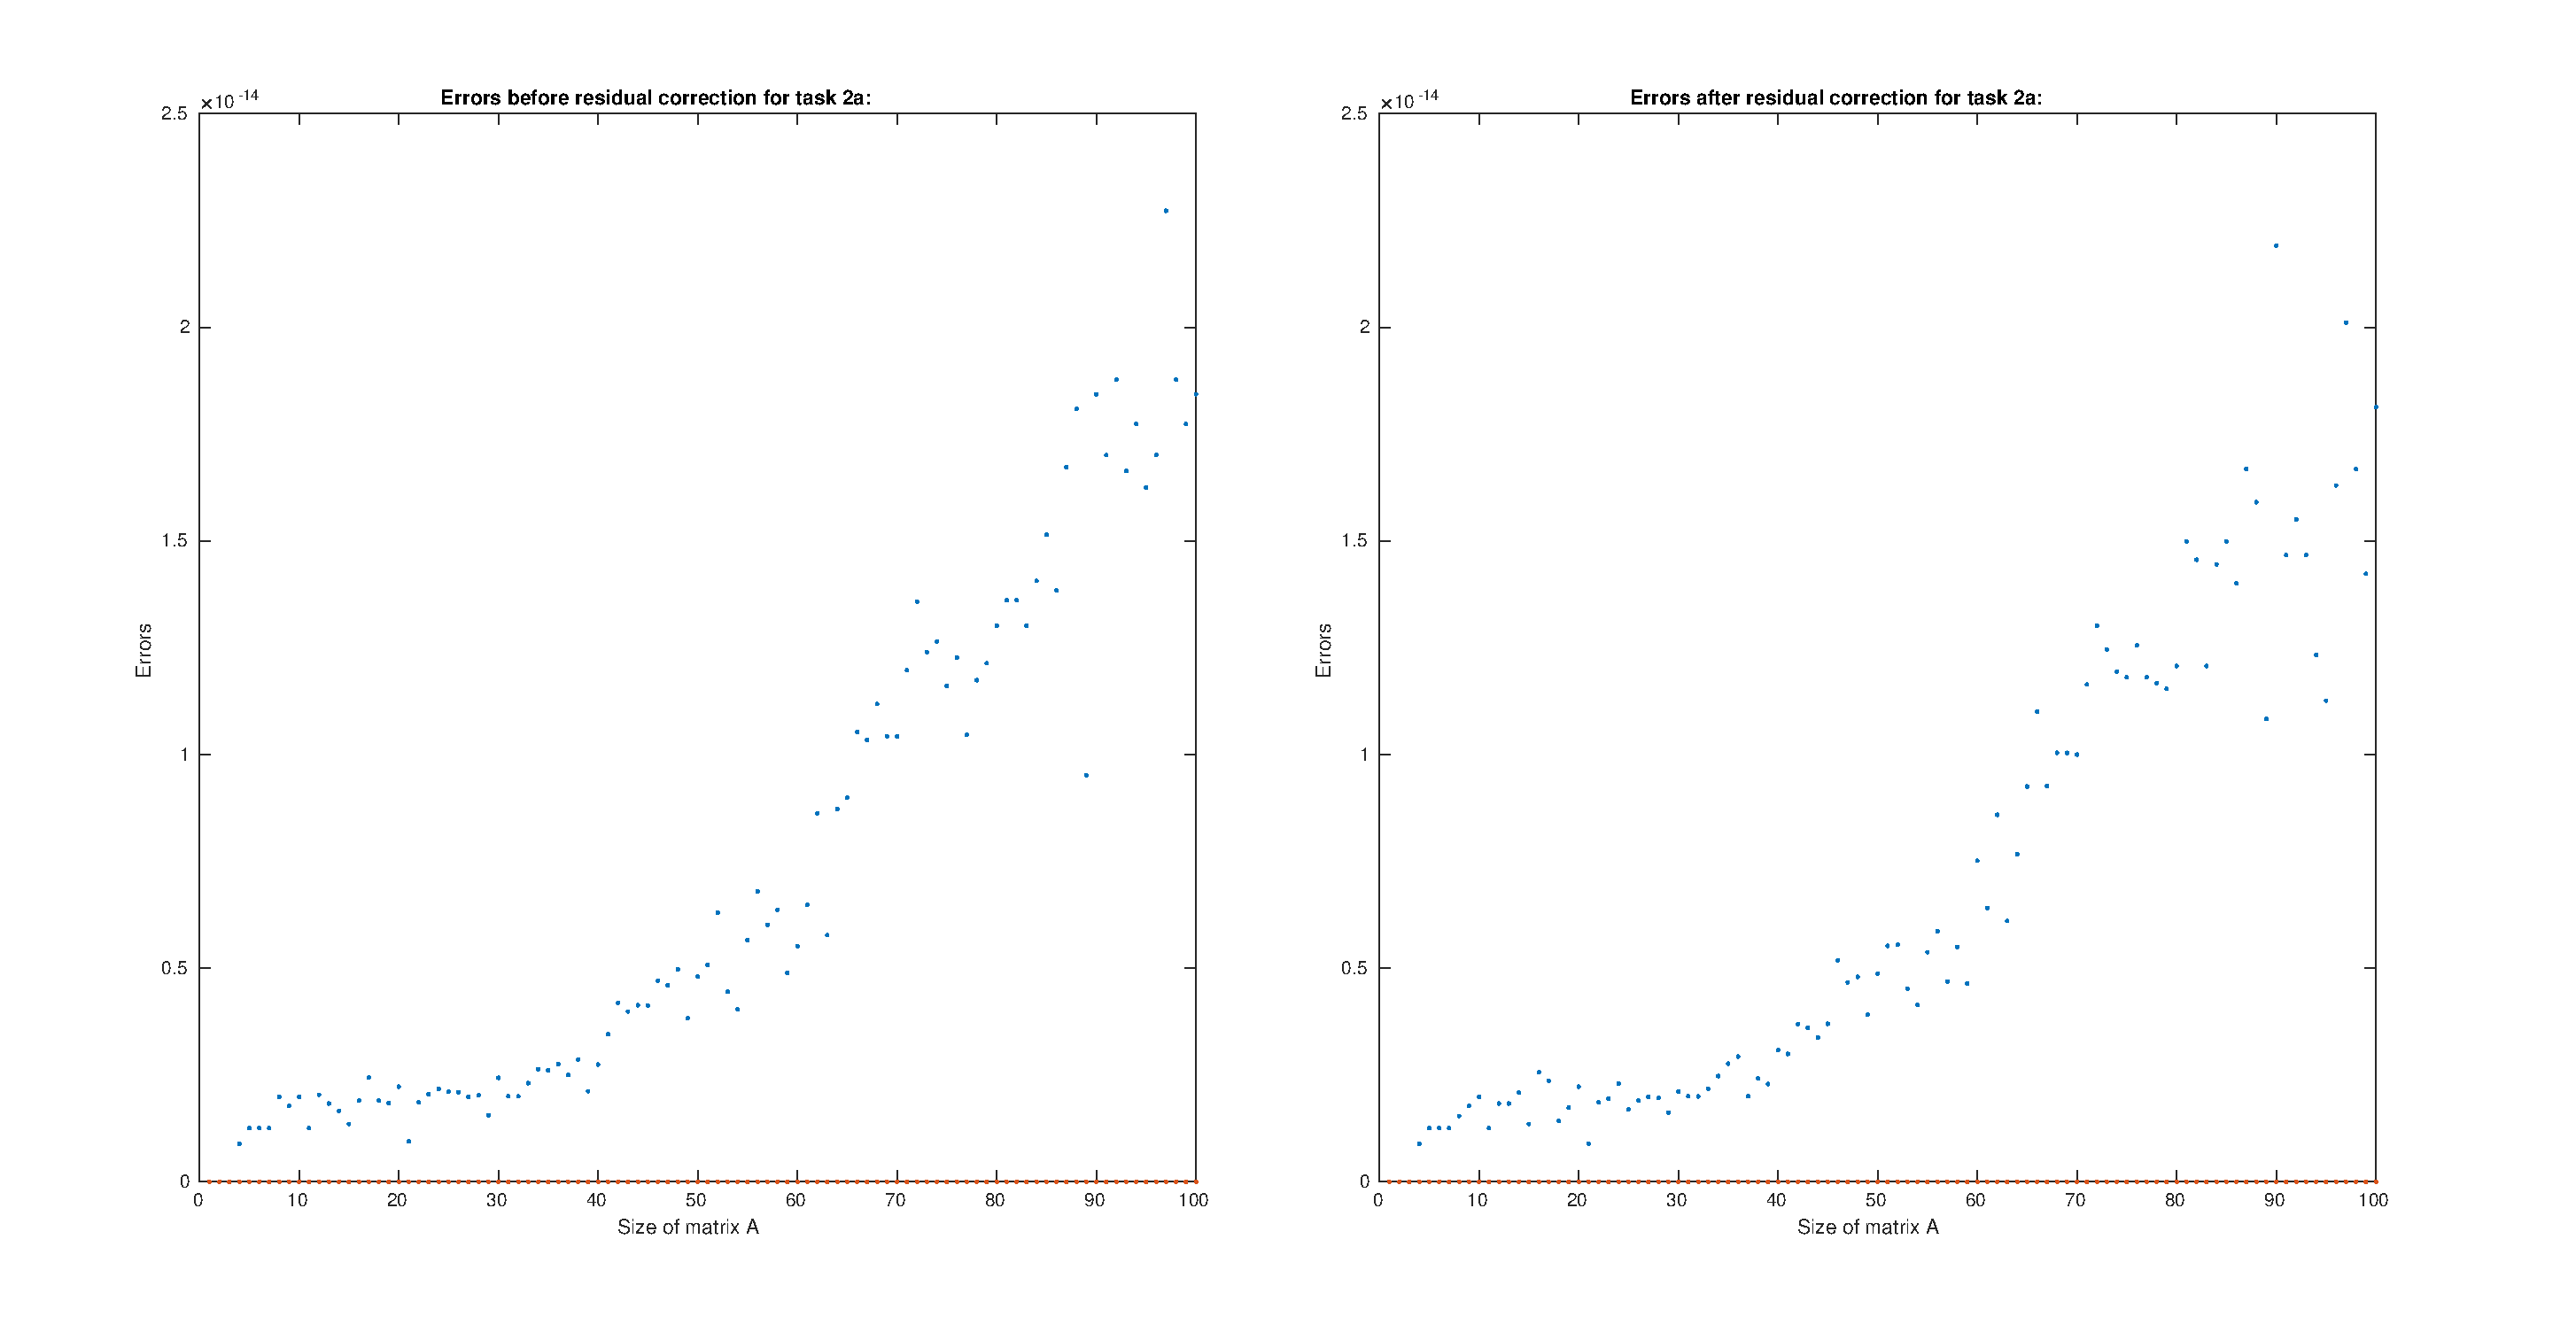
\includegraphics[scale=0.75]{errorsA.eps}
\end{center}

\begin{center}
   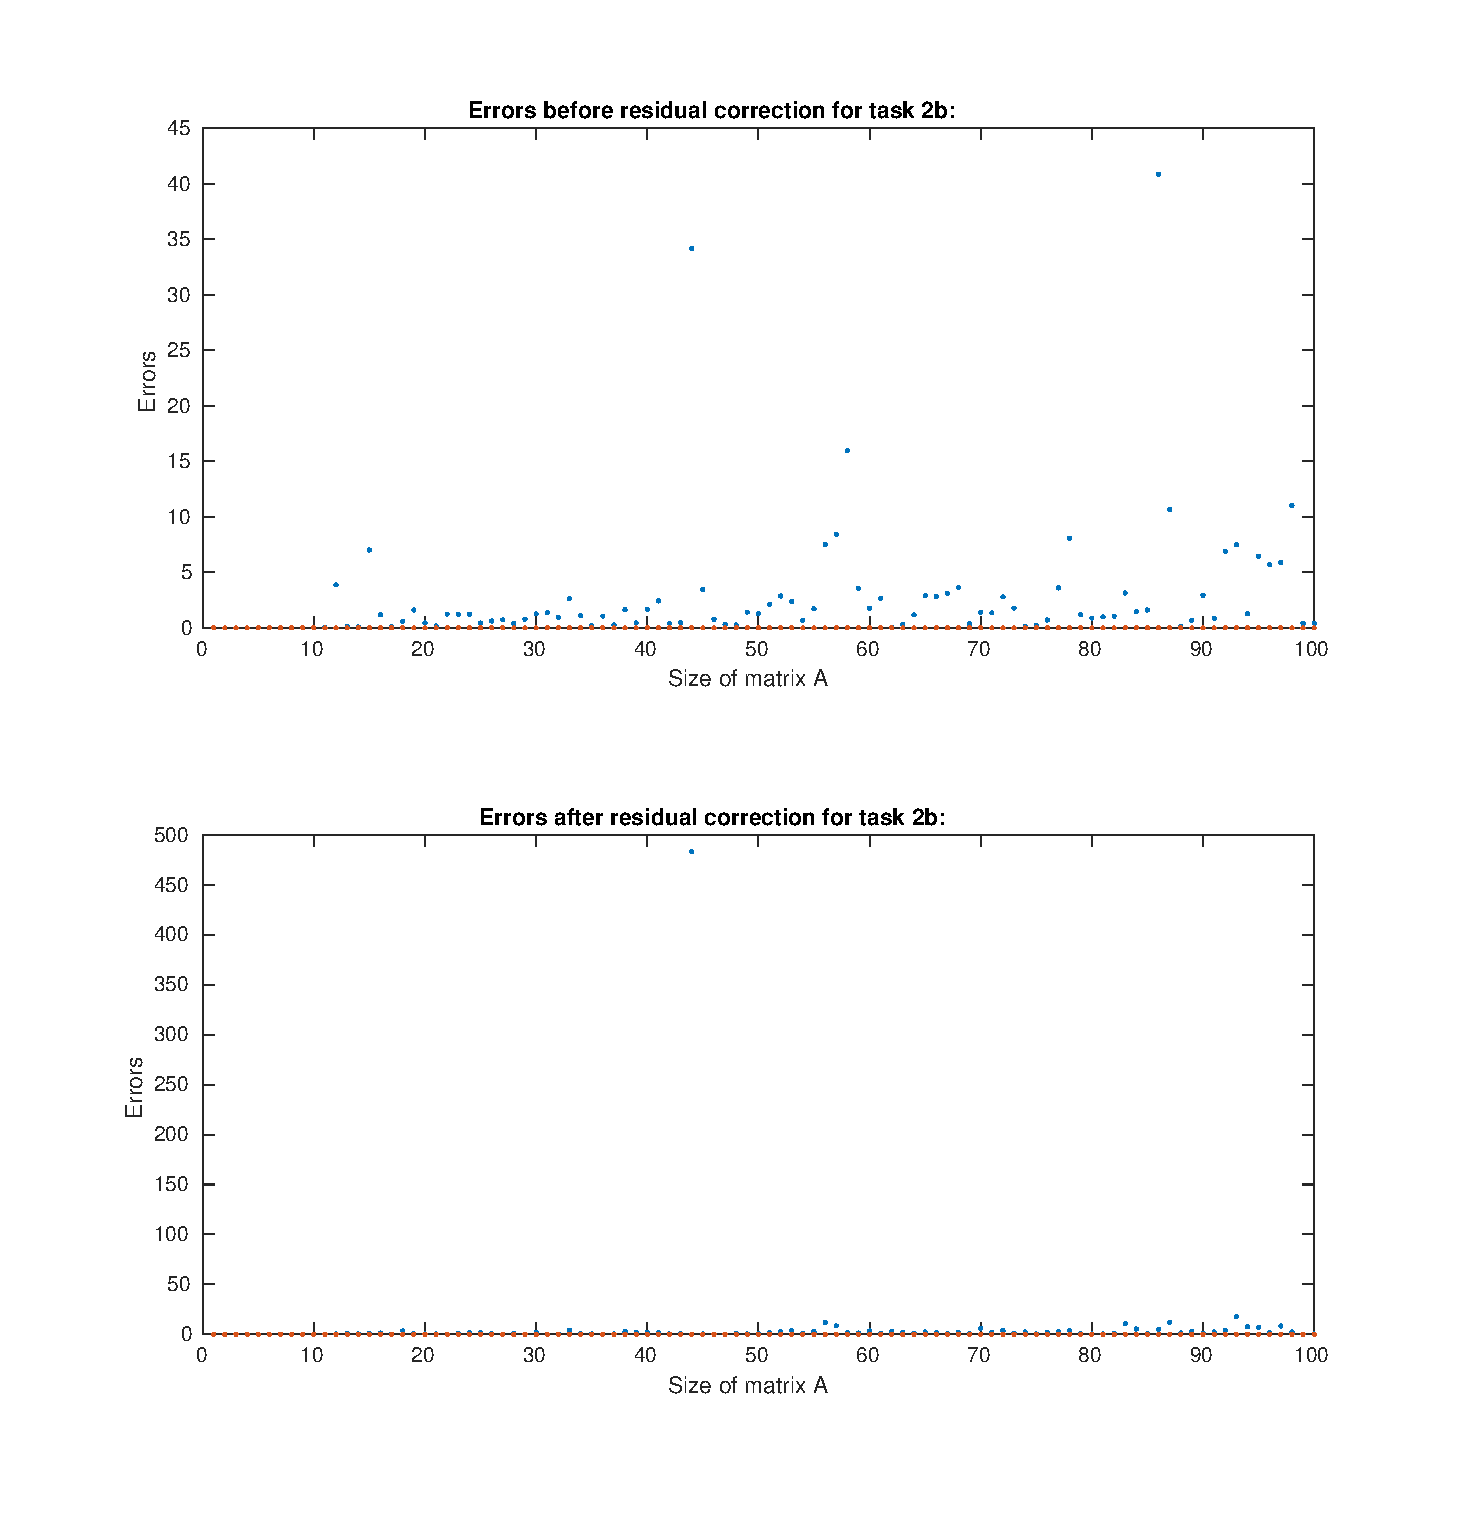
\includegraphics[scale=0.75]{errorsB.eps}
\end{center}
As we can see our residual correction method \textbf{does} work for Matrix B and Vector B and decreases the error drastically.

\subsection{Errors in b)}
Matrix B suffers from relatively huge errors. Where do they come from?
Matrix B is a variant of Hilbert matrix.
Equation for generating elements of this matrix is as follows:
\[ b_{ij} = \frac{5}{8(i + j + 1)} \]
Equation for generating elements of the Hilbert matrix is as follows:
\[ b_{ij} = \frac{1}{(i + j - 1)} \]
The only thing that changes are the constants, we have 5 instead of 1 in the numerator and 8 in front of the summation in the denominator and +1 instead of -1. For sufficiently huge 'i' and 'j' those differences hardly matter.
Hilbert matrix is badly conditioned. It's condtion number for \textit{n} size hilbert matrix is equal to:
\[ \mathcal{O}(\frac{e^{3.5255n}}{sqrt(n)}) \]
Let's calculate condition number of matrix B in matlab:
\begin{simplechar}
\begin{lstlisting}
cond(matrixB(10))
ans = 2.428027097978043e+14
\end{lstlisting}
\end{simplechar}

And compare it with condition number of matrix A:
\begin{simplechar}
\begin{lstlisting}
cond(matrixA(10))
ans = 4.550344127923193
\end{lstlisting}
\end{simplechar}
As we can see the difference is huge, conditon number of matrix B for 10 elements is $10^{14}$ times bigger than for matrix A. This explains big errors for matrix B.











\addtocontents{toc}{\protect\newpage}
\chapter{Problem 3 - Solving a system of n linear equations - iterative algorithm}

\section{Problem}
Write a general program for solving the system of n linear equations Ax = b using the Gauss-Seidel \textbf{and} Jacobi iterative algorithms.

We are given following system:
\[
\systeme{10x_1-4x_2+x_3+2x_4=-8, 2x_1-6x_2+3x_3-x_4=-12, x_1+4x_2-12x_3+x_4=4, 2x_1+3x_2-3x_3-10x_4=1}
\]

Then We need to compare the results of iterations plotting norm of the solution error versus the iteration number \textbf{k}, untill We get accuracy better than $10^{-10}$.

We should also try to solve the equations from problem 2a) and 2b) for n = 10 using iterative method of our choice.


\section{Theoretical introduction}

 We should also answer the question what happens if the sufficient condition is not fullfiled.

Itertaive methods differ from the Gauss elimination method since they are iterative, which means that our solution will improve with each iteration. Building on that We can cnclude that the number of iterations will depend on what accuracy We want to achieve. Since We are using iterative method We don't have the guarantee of how many iterations will be neeeded before We reach the solution,

In general:
We start with:
 \textbf{$x^{(0)}$ } - being the best known approximation of the solution point

And We generate next vectors  \textbf{$x^{i+1}$}  in such way:
\[ \mathbf{x^{i+1}} = \mathbf{M}\mathbf{x^{(i)}} + \mathbf{w} \]

Where $\mathbf{M}$ is some matrix.

\subsection{Procedure}

\subsubsection{Decomposing matrix}
For both Jacobi and Gauss-Seidel method We first decompose starting matrix $ \mathbf{A} $ to:
\[ \mathbf{A} = \mathbf{L} + \mathbf{D} + \mathbf{U} \]
where:
$ \mathbf{L} $ - Subdiagonal matrix
$ \mathbf{D} $ - Diagonal matrix
$ \mathbf{U} $ - Matrix with entries over the diagonal.

For example:
For:
\[ \mathbf{A} = \begin{bmatrix}
2 & 3 & 3\\
1 & 2 & 3\\
1 & 1 & 2
\end{bmatrix}
\]

We can get:
\[ \mathbf{L} = \begin{bmatrix}
0 & 0 & 0\\
1 & 0 & 0\\
1 & 1 & 0
\end{bmatrix}
\]
\[ \mathbf{D} = \begin{bmatrix}
2 & 0 & 0\\
0 & 2 & 0\\
0 & 0 & 2
\end{bmatrix}
\]
\[ \mathbf{U} = \begin{bmatrix}
0 & 3 & 3\\
0 & 0 & 3\\
0 & 0 & 0
\end{bmatrix}
\]

so:

\[ \mathbf{A} = \mathbf{L} + \mathbf{D} + \mathbf{U} \]

\[
\begin{bmatrix}
2 & 3 & 3\\
1 & 2 & 3\\
1 & 1 & 2
\end{bmatrix}
=
\begin{bmatrix}
0 & 0 & 0\\
1 & 0 & 0\\
1 & 1 & 0
\end{bmatrix}
+
\begin{bmatrix}
2 & 0 & 0\\
0 & 2 & 0\\
0 & 0 & 2
\end{bmatrix}
+
\begin{bmatrix}
0 & 3 & 3\\
0 & 0 & 3\\
0 & 0 & 0
\end{bmatrix}
\]

\subsubsection{Jacobi's method}
After decomposing matrix We can write the system of equations
\[ \mathbf{A}\mathbf{x} = \mathbf{b} \]
in the form:
\[ \mathbf{D}\mathbf{x} = -(\mathbf{L}+\mathbf{U})\mathbf{x}+\mathbf{b}
\]

If We assume that diagonal entries of matrix \textbf{A} are nonzero, then matrix \textbf{D} is nonsingular therefore We can propose such an iterative method:
\[ \mathbf{x}^{i+1} = -\mathbf{D}^{-1}(\mathbf{L}+\mathbf{U})\mathbf{x}^{(i)}+\mathbf{D}^{-1}\mathbf{x}
\]
This is the Jacobi's method.
We can rewritte this equation in the form of \textit{n} independent scalar equations:

\[
{x}_j^{i+1} = -\frac{1}{d_{jj}}(
\sum^n_{k=1} (l_{jk} + u_{jk})x_k^{(i)}+b_j)
) \]
Where $d_{jj}$; $l_{jk}$;  $u_{jk}$ are the elements of the respective matrixes \textbf{D}, \textbf{L}, \textbf{U}

Thanks to this We can do those computations in paraller, totally or partially if We are using a computer that enables a parallelization of the computations.

\paragraph{Converging}
Jacobi's method is convergent if We have strong diagonal dominance of the matrix \textbf{A}


\subsubsection{Gauss-Seidel method}
After decomposing matrix We can write the system of equations
\[ \mathbf{A}\mathbf{x} = \mathbf{b} \]
in the form:
\[ (\mathbf{L}+\mathbf{D})\mathbf{x} = -\mathbf{U}\mathbf{x}+\mathbf{b}
\]
Again We assume that \textbf{D} is nonsingular, in doing so We propose following iterative method:
\[ \mathbf{D}\mathbf{x}^{(i+1)} = -\mathbf{L}\mathbf{x}^{(i+1)}-\mathbf{U}\mathbf{x}^{(i)}+\mathbf{b}
\]
Since matrix \textbf{L} is subdiagonal, provided that We organse the calculation of elements of the vector $x^{(i_1)}$ in a proper way, it does not hurt that $x^{(i_1)}$ is on the right side of the equation.
In order to organise the calculation in the correct way We:
First take into account the structure of matrixes \textbf{D} and \textbf{L}:
\[
\begin{bmatrix}
d_{11}x_1^{(i_1)}\\
d_{22}x_2^{(i_1)}\\
d_{33}x_3^{(i_1)}\\
\vdots\\
d_{nn}x_n^{(i_1)}
\end{bmatrix}
=
-
\begin{bmatrix}
0 & 0 & 0 & \cdots & 0\\
l_{21} & 0 & 0 & \cdots & 0\\
l_{32} & l_{32} & 0 & \cdots & 0\\
\vdots & \vdots & \vdots & \vdots & \vdots\\
l_{n1} & l_{n2} & l_{n3} & \cdots & 0
\end{bmatrix}
\begin{bmatrix}
x_1^{(i_1)}\\
x_2^{(i_1)}\\
x_3^{(i_1)}\\
\vdots\\
x_n^{(i_1)}
\end{bmatrix}
-
\mathbf{w}^{(i)}
\]
Where
\[ \mathbf{w}^{(i)} = \mathbf{U}\mathbf{x}^{(i)} - \mathbf{b} \]

\newpage
So the order of calculations is as follows:
\[ x_1^{(i+1)} = -\frac{w_1^{(i)}}{d_{11}} \]
\[ x_2^{(i+1)} = -\frac{-l_{21}x_1^{(i+1)} - w_2^{(i)}}{d_{22}} \]
\[ x_3^{(i+1)} = -\frac{-l_{31}x_1^{(i+1)} -l_{32}x_2^{(i+1)} - w_3^{(i)}}{d_{33}} \]

And so on

As opposed to Jacobi's method, Gauss-Seidel method computations must be performed sequentially. Every subsequent scalar equations uses results from the computation of the previous equations.
\paragraph{Converging}
Gauss-Seidel method is convergent if the matrix \textbf{A} is strongly row or column diagonnaly dominant. If the matrix is symmetric, the method is also convergent if the matrix \textbf{A} is positive definite. This method is also usually faster convergent compared to Jacobi's method.

\subsubsection{Stop tests}
There are two ways to check when to terminate iterations of the methods We just discussed:
\begin{enumerate}
\item Check differences between two subsequent iteration points
\[
\| \mathbf{x}^{(i+1)} - \mathbf{x}^{(i)} \| \leq \delta
\]
Where $\delta$ is an assumed tolerance, (in our case $10^{-10}$). What We are really interested in though is whether the solution of the system of equation has required accuracy. If We want to check that We can additionaly check (higher level, more computationally demanding test):
\item Check differences between two subsequent iteration points
\[
\| \mathbf{A}\mathbf{x}^{(i+1)} - \mathbf{b}\| \leq \delta_2
\]
Where $\delta_2$ is an assumed tolerance. If this test is not passed then We can diminish the value of $\delta_2$ and continue with the iterations. Value of $\delta_2$ can not be too small since We are limited by the numerical errors.
\end{enumerate}

\subsubsection{\textbf{A} and \textbf{b}}
We have been given the following system:
\[
\systeme{10x_1-4x_2+x_3+2x_4=-8, 2x_1-6x_2+3x_3-x_4=-12, x_1+4x_2-12x_3+x_4=4, 2x_1+3x_2-3x_3-10x_4=1}
\]
Therefore our matrices will look like this:
\[
\textbf{A} = \begin{bmatrix}
10 & -4 & 1 & 2 \\
2 & -6 & 3 & -1 \\
1 & 4 & -12 & 1 \\
2 & 3 & -3 & -10
\end{bmatrix}
\textbf{b} = \begin{bmatrix}
-8 \\
-12 \\
4 \\
11 \\
\end{bmatrix}
\]

So:
\[
\textbf{L} = \begin{bmatrix}
0 & 0 & 0 & 0 \\
2 & 0 & 0 & 0 \\
1 & 4 & 0 & 0 \\
2 & 3 & -3 & 0
\end{bmatrix}
\textbf{D} = \begin{bmatrix}
10 & 0 & 0 & 0 \\
0 & -6 & 0 & 0 \\
0 & 0 & -12 & 0 \\
0 & 0 & 0 & -10
\end{bmatrix}
\textbf{U} = \begin{bmatrix}
0 & -4 & 1 & 2 \\
0 & 0 & 3 & -1 \\
0 & 0 & 0 & 1 \\
0 & 0 & 0 & 0
\end{bmatrix}
\]
\[
\textbf{D}^{-1} = \begin{bmatrix}
\frac{1}{10} & 0 & 0 & 0 \\
0 & - \frac{1}{6} & 0 & 0 \\
0 & 0 & - \frac{1}{12} & 0 \\
0 & 0 & 0 & - \frac{1}{10}
\end{bmatrix}
\]

\section{Results}

\subsection{Jacobi method result}
For system of equations We got in this task We got following results:
\\
Without the change in demanded tolerance:
\[ x = \left( \begin{array}{cc}
  -0.076776098668341 \\
   2.105784262642568 \\
   0.395344797635474 \\
   0.397776619764909
\end{array} \right)
\]
Error:
\[ r = \| \mathbf{A}\mathbf{x} - \mathbf{b}\| = 1.154375287358407e-10 \]
We managed to do this in \textbf{38} iterations of our loop, and the demanded tolerance did not change. (This required small change in code where We ommited the part of code responsible for changing demandedTolerance if $ \| \mathbf{A}x-b \| > \delta_2) $ )

With the change in demanded tolerance:
\[ x = \left( \begin{array}{cc}
  -0.076776098668341 \\
   2.105784262642568 \\
   0.395344797635474 \\
   0.397776619764909
\end{array} \right)
\]
Error:
\[ r = \| \mathbf{A}\mathbf{x} - \mathbf{b}\| = 5.770361548895147e-11 \]
We got this result in \textbf{37} iterations and demanded tolerance was equal to $2*10^{-10}$

Compared to matlab function
\[ x_{matlab} = \left( \begin{array}{cc}
  -0.076776098662498 \\
   2.105784262636790 \\
   0.395344797637659 \\
   0.397776619767240 \\
\end{array} \right)
\]
Matlab error:
\[ r = \| \mathbf{A}\mathbf{x} - \mathbf{b}\| = 4.070144838902081e-15 \]

For data from task 2a We got: \\
Without change in demanded tolerance:
\[ x_a = \left( \begin{array}{cc}
-0.930024655108186 \\
-1.223407298660663 \\
-1.273530574212508 \\
-1.230517757317628 \\
-1.151356031082747 \\
-1.056883669273682 \\
-0.952628310081466 \\
-0.834334594312996 \\
-0.683708806198363 \\
-0.450125157620744 \\
\end{array} \right)
\]
Error:
\[ r = \| \mathbf{A}\mathbf{x} - \mathbf{b}\| = 6.955194519943778e-11 \]
We managed to do this in \textbf{59} iterations of our loop, and the demanded tolerance did not change.

With change in demanded tolerance:
\[ x_a = \left( \begin{array}{cc}
-0.930024655104470 \\
-1.223407298653515 \\
-1.273530574202540 \\
-1.230517757305602 \\
-1.151356031069692 \\
-1.056883669260597 \\
-0.952628310069469 \\
-0.834334594303006 \\
-0.683708806191233 \\
-0.450125157617020 \\
\end{array} \right)
\]
Error:
\[ r = \| \mathbf{A}\mathbf{x} - \mathbf{b}\| = 1.699812218689508e-10 \]
We managed to do this in \textbf{57} iterations of our loop, and the demanded tolerance changed to $4*10^{-10}$

Compared to matlab $ A \ b $ function
\[ x_{matlab} = \left( \begin{array}{cc}
  -0.930024655110760 \\
  -1.223407298665612 \\
  -1.273530574219411 \\
  -1.230517757325956 \\
  -1.151356031091789 \\
  -1.056883669282743 \\
  -0.952628310089775 \\
  -0.834334594319914 \\
  -0.683708806203301 \\
  -0.450125157623323 \\
\end{array} \right)
\]
Matlab error:
\[ r = \| \mathbf{A}\mathbf{x} - \mathbf{b}\| = 3.662053438817790e-15 \]

For Matrix and Vector from task 2b) error of
\[ \| x^{(i+1)} - x^{(i)} \| \]
grew to infinity, therefore We could never achieve demanded tolerance, therefore the program executed infinite loop.

\subsubsection{Minimizing the demanded error}
We tried to minimize the demanded error using this steps:
\begin{enumerate}
\item We copied error from matlab function and pasted it into demanded tolerance.
\item If We did not get infinite loop We copied the newly acquired error and pasted it into demanded tolerance.
\item If We got inifinite loop We used the previous error as "minimal" demanded error.
\end{enumerate}
\paragraph{For original system of equations:}
We managed to get results with error as low as $1.776356839400250e-15$ with demanded tolerance = $3.202372833989376e-15$ for lower values program went into infinite loop.
Results for demanded tolerance = $3.202372833989376e-15$
For given matrix:
\[ x = \left( \begin{array}{cc}
  -0.076776098662498 \\
   2.105784262636790 \\
   0.395344797637659 \\
   0.397776619767240
\end{array} \right)
\]
Error:
\[ r = \| \mathbf{A}\mathbf{x} - \mathbf{b}\| = 3.108624468950438e-15 \]
We got this result in \textbf{53} iterations and demanded tolerance did not change.

\paragraph{For task 2a) system of equations:}
We managed to get results with error as low as
\[ 3.108624468950438e-15 \] with demanded tolerance:
\[ 3.202372833989376e-15 \]
for lower values program went into infinite loop.

For demanded tolerance = $3.202372833989376e-15$:
Results for 2a) system of equation

\[ x_a = \left( \begin{array}{cc}
-0.930024655110760 \\
-1.223407298665613 \\
-1.273530574219411 \\
-1.230517757325955 \\
-1.151356031091788 \\
-1.056883669282743 \\
-0.952628310089775 \\
-0.834334594319914 \\
-0.683708806203301 \\
-0.450125157623323
\end{array} \right)
\]
Error:
\[ r = \| \mathbf{A}\mathbf{x} - \mathbf{b}\| = 3.108624468950438e-15 \]
We managed to do this in \textbf{84} iterations of our loop, and the demanded tolerance did not change.
We managed to achieve slightly better (as in, the error was smaller) results than Matlab custom function.

\subsection{Gauss-Seidel method result}
For system of equations We got in this task We got following results:
\\
\[ x = \left( \begin{array}{cc}
  -0.076776098752996 \\
   2.105784262542701 \\
   0.395344797589652 \\
   0.397776619735316
\end{array} \right)
\]
Error:
\[ r = \| \mathbf{A}\mathbf{x} - \mathbf{b}\| = 6.999102842719934e-10 \]
We managed to do this in \textbf{19} iterations of our loop, and the demanded tolerance did not change.
Error:
\[ r = \| \mathbf{A}\mathbf{x} - \mathbf{b}\| = 6.999102842719934e-10 \]
We got this result in \textbf{19} iterations and demanded tolerance was equal to $2*10^{-10}$

For data from task 2a We got: \\
\[ x_a = \left( \begin{array}{cc}
-0.930024655049330 \\
-1.223407298590161 \\
-1.273530574151901 \\
-1.230517757273947 \\
-1.151356031055568 \\
-1.056883669259564 \\
-0.952628310076145 \\
-0.834334594312669 \\
-0.683708806199986 \\
-0.450125157622217 \\
\end{array} \right)
\]
Error:
\[ r = \| \mathbf{A}\mathbf{x} - \mathbf{b}\| = 5.311669113699570e-10 \]
We managed to do this in \textbf{28} iterations of our loop, and the demanded tolerance did not change.

For Matrix and Vector from task 2b) error of
\[ \| x^{(i+1)} - x^{(i)} \| \]
grew to infinity, therefore We could never achieve demanded tolerance, therefore the program executed infinite loop.

\subsubsection{Minimizing the demanded error}
I tried to minimize the demanded error using this steps:
\begin{enumerate}
\item I copied error from matlab function and pasted it into demanded tolerance.
\item If I did not get infinite loop I copied the newly acquired error and pasted it into demanded tolerance.
\item If I got inifinite loop I used the previous error as "minimal" demanded error.
\end{enumerate}
\paragraph{For original system of equations:}
We managed to get results with error as low as $1.776356839400250e-15$ with demanded tolerance = $ 1.986027322597818e-15 $ for lower values program went into infinite loop.
Results for demanded tolerance = $1.986027322597818e-15$
For given matrix:
\[ x = \left( \begin{array}{cc}
  -0.076776098662498 \\
   2.105784262636790 \\
   0.395344797637659 \\
   0.397776619767240
\end{array} \right)
\]
Error:
\[ r = \| \mathbf{A}\mathbf{x} - \mathbf{b}\| = 1.776356839400250e-15 \]
We got this result in \textbf{30} iterations and demanded tolerance did not change.

\paragraph{For task 2a) system of equations:}
We managed to get results with error as low as
\[ 1.538370149106851e-15 \] with demanded tolerance:
\[ 1.538370149106851e-15 \]
for lower values program went into infinite loop.

For demanded tolerance = $1.538370149106851e-15$:
Results for 2a) system of equation

\[ x_a = \left( \begin{array}{cc}
-0.930024655110760 \\
-1.223407298665613 \\
-1.273530574219411 \\
-1.230517757325955 \\
-1.151356031091788 \\
-1.056883669282743 \\
-0.952628310089775 \\
-0.834334594319914 \\
-0.683708806203301 \\
-0.450125157623323 \\
\end{array} \right)
\]
Error:
\[ r = \| \mathbf{A}\mathbf{x} - \mathbf{b}\| = 1.538370149106851e-15 \]
We managed to do this in \textbf{42} iterations of our loop, and the demanded tolerance did not change.
We managed to achieve slightly better (as in, the error was smaller) results than Matlab custom function.

\paragraph{Table}

\begin{center}
\resizebox{\textwidth}{!}{
\begin{tabular}{||c c c c c c||}
 \hline
 system of equations & method & demanded tolerance & error & iterations \\
 \hline
 task 3 system & Jacobi method & 10e-10 & 1.154375287358407e-10 & 38 \\
 \hline
 task 3 system & Jacobi method & 10e-10 & 5.770361548895147e-11 & 37 \\
 \hline
 task 3 system & Jacobi method & 3.202372833989376e-15 & 3.108624468950438e-15 & 53 \\
 \hline
 task 3 system & Gaussian-Seidel method & 10e-10 & 6.999102842719934e-10 & 19 \\
 \hline
 task 3 system & Gaussian-Seidel method & 1.776356839400250e-15 & 1.776356839400250e-15 & 30 \\
 \hline
 task 3 system & Matlab function & ? & 4.070144838902081e-15 & ? \\
 \hline
 task 2a) system & Jacobi method & 10e-10 & 6.955194519943778e-11 & 59 \\
 \hline
 task 2a) system & Jacobi method & 10e-10 & 1.699812218689508e-10 & 57 \\
 \hline
 task 2a) system & Jacob method & 3.202372833989376e-15 & 3.108624468950438e-15 & 84 \\
 \hline
 task 2a) system & Gaussian-Seidel method & 10e-10 & 5.311669113699570e-10 & 28 \\
 \hline
 task 2a) system & Gaussian-Seidel method & 1.538370149106851e-15 & 1.538370149106851e-15 & 42 \\
 \hline
 task 2a) system & Matlab function & ? & 3.662053438817790e-15 & ? \\
 \hline

\end{tabular}}
\end{center}

\section{Discussion of results}
\subsection{Comparison based on table}
Gaussian-Seidel method takes less iterations, can achieve smaller error and works under smaller demanded tolerance, that being said Jacobi method has one crucial advantage - it can be run in parallel. That means that even when Jacobi method takes twice or thrice amount of iteration us Gaussian-Seidel one if we just run it in paraller we can diminish this difference. In the examples we worked in, just two jacobi method running in paraller provide us with similar amount of iterations per one process as in Gaussian-Seidel one, and three or more processes give the edge to Jacobi method. With modern CPU's with at least 5 cores and correct implementation of algorithm, jacobi method reigns supreme.

\subsection{Convergence}
The biggest problem is of course the fact that those iterative methods do not work on every system of equation. Like the one from task 2b).
For Jacobi's method the matrix is convergent if it has strong diagonal dominance. \textbf{A}, i.e:
\begin{enumerate}
  \item \[ \| a_{ii} \| > \sum^n_{j=1, j \neq i} \|a_{ij} \| \]
  \item \[ \| a_{jj} \| > \sum^n_{i=1, i \neq j} \|a_{ij} \| \]
\end{enumerate}
For Gaussian-Seidel method the matrix is convergent if it has strong diagonal dominance \textbf{or} if the matrix \textbf{A} is symmetric and positivie definite.
\subsubsection{2b) task convergence }
Let's check strong diagonal dominance from matrix \textbf{A} from task 2b) in matlab:
\begin{simplechar}
\begin{lstlisting}
function d = checkIfDiagonallyDominant(Matrix)
    d = 1;
    [Rows, ~] = size(Matrix);
    for i = 1 : Rows
        rowsSum = 0;
        for j = 1 : Rows
            rowsSum = rowsSum + abs(Matrix(i, j));
        end
        rowsSum = rowsSum - Matrix(i, i);
        if Matrix(i, i) <= rowsSum
            d = 0;
            break
        end
    end
end
\end{lstlisting}
\end{simplechar}
checkIfDiagonallyDominant(matrixB(10)) returns '0', therefore matrix from task 2b) will \textbf{not} converge. And as expected it does not work when put in my jacobiLoop function.
\subsubsection{Iterations as function of size of Matrix}
I have used matrix from task 2a), demanded tolerance equal to 10e-10, and max size of matrix equal to 500. for both methods
\begin{center}
   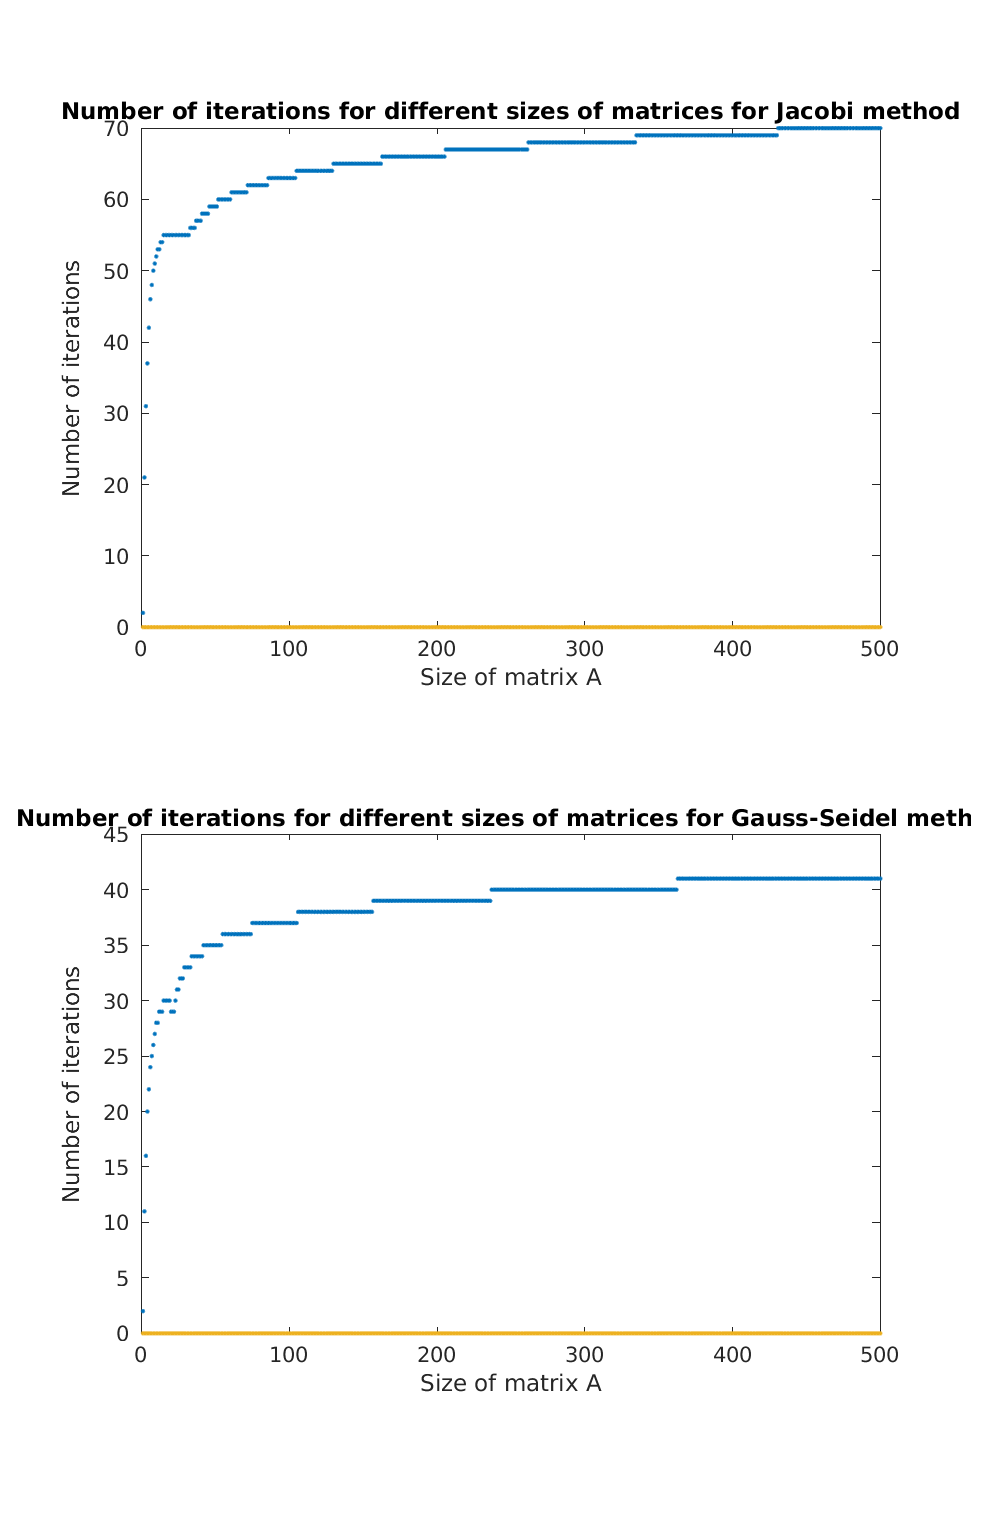
\includegraphics[scale=0.75]{iterations.eps}
\end{center}
Gauss Seidel method again requires fewer iterations, around half the amount for jacobi method. For both methods number of iterations acts like logarithmic function. Therefore we can assume that for big matrices required number of iterations will not change so drastically.

\chapter{Problem 4 - QR method of finding eigenvalues}

\section{Problem}
We must find eigenvalues of 5x5 matrices. Both without shifts and with shifts.
\section{Theoretical introduction}
\subsection{Eigenvalues}
Eigenvalues of matrix \textbf{A} are defined as a pair of number $\lambda$ and vector \textbf{v} such that:
\[ \mathbf{A}\mathbf{v} = \lambda\mathbf{v} \]
This can be rewritten as:
\[ (\mathbf{A} - \lambda\mathbf{I})\mathbf{v} = 0 \]
And further we get characteristic equation:
\[ det(\mathbf{A} - \lambda\mathbf{I}) = 0 \]

\subsection{QR method for finding eigenvalues}
First we start by transforming matrix \textbf{A} into tridiagonal form. It increases the effectiveness of calculations.

Single step of QR method consists of:
\[ \textbf{A}^{(k)} = \textbf{Q}^{(k)}\textbf{R}^{(k)} \]
\[ \textbf{A}^{(k+1)} = \textbf{R}^{(k)}\textbf{Q}^{(k)} \]
$\textbf{Q}^{(k)}$ being orthogonal, therefore:
\[ \textbf{R}^{(k)} = (\textbf{Q}^{(k)}))^{-1}\textbf{A}^{(k)} = \textbf{Q}^{(k)T}\textbf{A}^{(k)}\textbf{Q}^{(k)} \]
therefore:
\[ \textbf{A}^{(k+1)} = \textbf{Q}^{(k)T}\textbf{A}^{(k)}\textbf{Q}^{(k)} \]
If we have symmetric matrix \textbf{A} it converges to the diagonal matrix $diag(\lambda_i)$

Since this method can be slowly convergent we use shifts. Single iteration of QR method with shifts looks like this:
\begin{equation}
\begin{split}
\textbf{A}^{(k)} - p_k\textbf{I} &= \textbf{Q}^{(k)}\textbf{R}^{(k)} \\
\textbf{A}^{(k+1)} &= \textbf{R}^{(k)}\textbf{Q}^{(k)} + p_k\textbf{I} \\
&= \textbf{Q}^{(k)T}(\textbf{A}^{(k)} - p_k\textbf{I})\textbf{Q}^{(k)} + p_k\textbf{I} \\
&=\textbf{Q}^{(k)T}\textbf{A}^{(k)}\textbf{Q}^{(k)} \\
\end{split}
\end{equation}

Wher $p_k$ should be chosen as a best estimate of $\lambda_{i+1}$

\section{Results}
\subsection{Starting matrix}
I decided to generate random symmetric matrix using following code:
\begin{simplechar}
\begin{lstlisting}
function A = matrix4()
    A = 10 * rand(5); % rand generates 5x5 matrix filled with random numbers
    % we multiply by 10 to get at lest one digit in front of the dot
    A = floor(A); % we floor the matrix we got to get nice natural numbers matrix
    A = A * A'; % we get symmetric matrix
    disp(issymmetric(A)); % we check if matrix is symmetric
end
\end{lstlisting}
\end{simplechar}
I got the following matrix:
\[
\begin{bmatrix}
171  &  48  & 133  &  81  &  93 \\
 48  & 108  &  63  &  35  &  30 \\
133  &  63  & 131  &  64  &  91 \\
 81  &  35  &  64  &  41  &  37 \\
 93  &  30  &  91  &  37  & 106
\end{bmatrix}
\]

Putting it through Matlab eig function I got eigen values equal to:
\[
10^{2} *
\begin{bmatrix}
  0.000050598692964 \\
  0.105696602175690 \\
  0.454589544003707 \\
  0.870708987227002 \\
  4.138954267900641
\end{bmatrix}
\]


\subsection{QR method with no shifts}
Putting this matrix to my functions QRNoShifts and QRShifts I got:
for qr method with no shifts:
Final matrix:
\[
\begin{bmatrix}
413.8954  &  0.0000  & -0.0000  &  0.0000  &  0.0000 \\
 0.0000  & 87.0709  &  -0.0000  &  -0.0000  &  0.0000 \\
0.0000  &  -0.0000  & 45.4590  &  -0.0000  &  -0.0000 \\
 -0.0000  &  0.0000  &  -0.0000  &  10.5697  &  -0.0000 \\
 0.0000  &  -0.0000  &  0.0000  &  0  & 0.0051
\end{bmatrix}
\]

Eigen values:
\[
10^{2} *
\begin{bmatrix}
  4.138954267900639 \\
   0.870708987227001 \\
   0.454589544003706 \\
   0.105696602175689 \\
   0.000050598692964 \\
\end{bmatrix}
\]

It took \textbf{26} iterations to get those values.

\subsection{QR method with shifts}
For qr method with shiftts:
Final matrix:
\[
\begin{bmatrix}
413.8954
\end{bmatrix}
\]

Eigen values:
\[
10^{2} *
\begin{bmatrix}
  0.454589544003706 \\
  0.870708987227001 \\
  0.105696602175689 \\
  0.000050598692964 \\
  4.138954267900639
\end{bmatrix}
\]

It took \textbf{12} iterations to get those values.

\section{Discussion of the result}
Following plot was generated using task4Plot function, using maxMatrixSize = 25 and generating random symmetrical matrix of size i x i in each loop. Both QR methods were given exactly the same matrices.
\subsection{Plot}

\begin{center}
   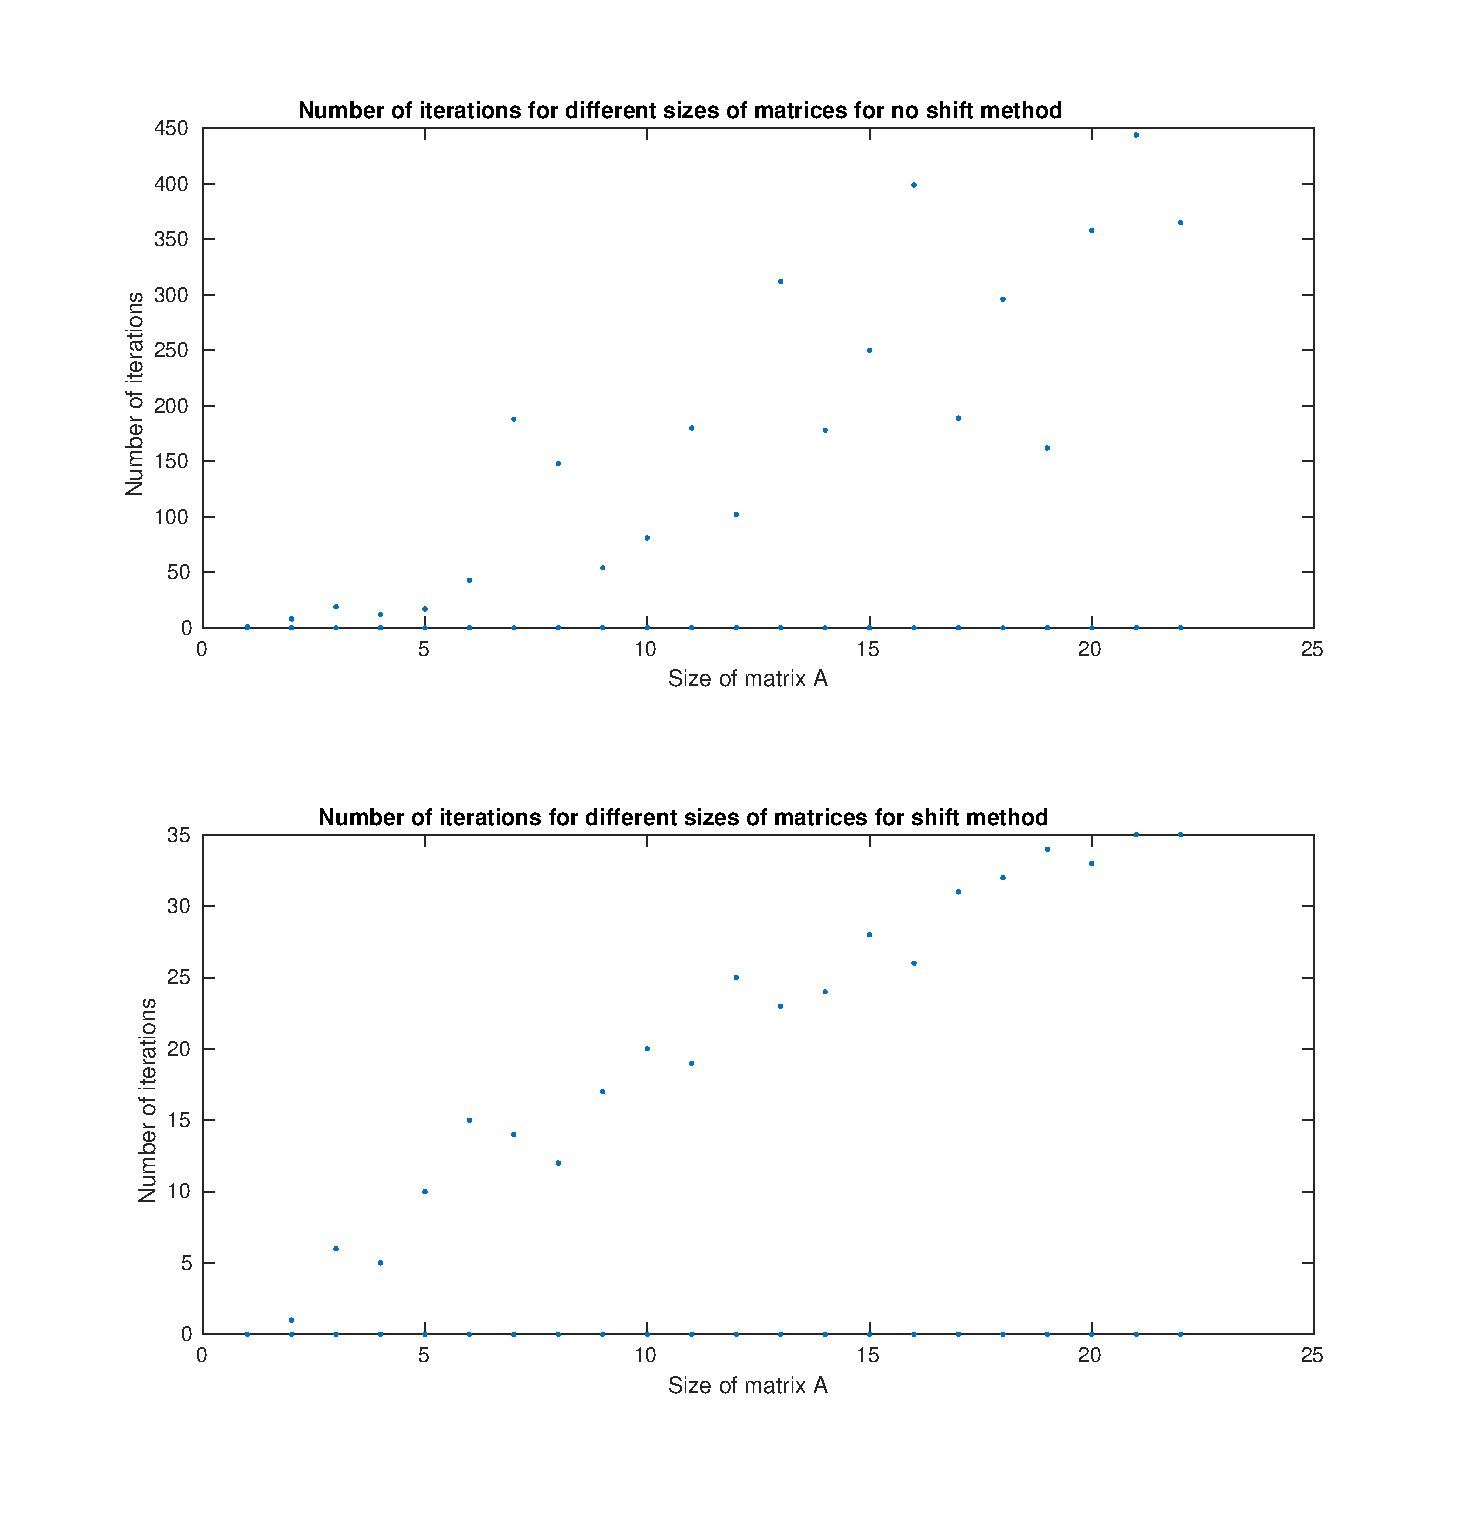
\includegraphics[scale=0.5]{task4plot.eps}
\end{center}
\subsection{Shift method superiority}
As we can see:
QR method with shifts is much more efficient and reliable.
\begin{enumerate}
\item For big enough matrices it requires ten times less iterations compared to QR method without shifts.
\item It is more efficient in our chosen matrix.
\item It can work with non-symetric matrices
\item Has no problem with generating complex eigen values.
\end{enumerate}
 One thing that does not change much is the precision, with both algorithms outputting similar results.







\chapter{Code appendix}

\section{Task 2 Code}

\subsection{Main function}
\begin{simplechar}
\begin{lstlisting}
function x = indicatedMethod(Matrix, Vector) % Name of the method as in the textbook
% x stands for obtained result
    [~,Columns] = size(Matrix); % We need to know how big the matrix is in next steps
    % notice the '~', since We assume We use square matrix, We do not need
    % to have another variable for number of rows since it is the same as
    % number of columns
    checkIfMatrixIsSquareMatrix(Matrix);
    [Matrix, Vector] = gaussianEliminationWithPartialPivoting(Columns, Matrix, Vector);
    % Change matrix to upper triangular matrix
    [Matrix, Vector, x] = backSubstitutionPhase(Columns, Matrix, Vector);
    % Get the solution
    x = iterativeResidualCorrection(Matrix, x, Vector); % Improve on the solution
end % end function
\end{lstlisting}
\end{simplechar}

\subsection{checkIfMatrixIsSquareMatrix}
\begin{simplechar}
\begin{lstlisting}
function checkIfMatrixIsSquareMatrix(Matrix)
    [Rows,Columns] = size(Matrix);
    if Rows ~= Columns
        error ('Matrix is not square matrix!');
    end % end if
end % end function
\end{lstlisting}
\end{simplechar}

\newpage
\subsection{gaussianEliminationWithPartialPivoting}
\begin{simplechar}
\begin{lstlisting}
function [Matrix, Vector] = gaussianEliminationWithPartialPivoting(Columns, Matrix, Vector)
    for j = 1 : Columns
            centralElement = max(Matrix(j:Columns,j));
            % We stay in the same row (j) but We change columns, as in the
            % textbook
            [Matrix, Vector] = partialPivoting(Matrix, Vector, j, centralElement, Columns);
            % ensures that a_kk != 0 and reduces errors
            [Matrix, Vector] = gaussianElimination(j, Columns, Matrix, Vector);
            % change matrix into upper triangular matrix
    end % end for
end % end function
\end{lstlisting}
\end{simplechar}

\subsection{partialPivoting}
\begin{simplechar}
\begin{lstlisting}
function [Matrix, Vector] = partialPivoting(Matrix, Vector, j, centralElement, Columns)
    for k = j : Columns
        partialPivotingSwapOneRow(Matrix, Vector, j, k, centralElement);
    end % end for
end % end function
\end{lstlisting}
\end{simplechar}

\subsection{partialPivotingSwapOneRow}
\begin{simplechar}
\begin{lstlisting}
function [Matrix, Vector] = partialPivotingSwapOneRow(Matrix, Vector, j, k, centralElement)
    if Matrix(k,j) == centralElement
    swapRowMatrix(Matrix, j, k); % swap jth row with kth row
    swapValueVector(Vector, j, k); % swap jth value with kth value
    end % end if
end % end function
\end{lstlisting}
\end{simplechar}


\subsection{swapRowMatrix}
\begin{simplechar}
\begin{lstlisting}
function Matrix = swapRowMatrix(Matrix, j, k)
    temp =  Matrix(j , :); % ' : ' denote "all elements in jth row"
    Matrix(j , :) = Matrix(k, :);
    Matrix(k, :) = temp; % temp equal to previous value of jth row
end
\end{lstlisting}
\end{simplechar}

\subsection{swapValueVector}
\begin{simplechar}
\begin{lstlisting}
function Vector = swapValueVector(Vector, j, k)
    temp = Vector(j);
    Vector(j) = Vector(k);
    Vector(k) = temp;  % temp equal to previous value of k element of vector
end % end function
\end{lstlisting}
\end{simplechar}

\subsection{gaussianElimination}
\begin{simplechar}
\begin{lstlisting}
function [Matrix, Vector] = gaussianElimination(j, Columns, Matrix, Vector)
    for i = j + 1 : Columns
        rowMultiplier = Matrix(i,j) / Matrix(j,j);
        [Matrix, Vector] = substractRows(Matrix, Vector, i, rowMultiplier, j, Columns);
    end % end for
end % end function
\end{lstlisting}
\end{simplechar}

\subsection{substractRows}
\begin{simplechar}
\begin{lstlisting}
function [Matrix, Vector] = substractRows(Matrix, Vector, i, rowMultiplier, j, Columns)
    Vector(i) = Vector(i) - rowMultiplier * Vector(j);
    for curentColumn = 1 : Columns
        Matrix(i,curentColumn) = Matrix(i,curentColumn) - rowMultiplier * Matrix(j, curentColumn);
    end % end for
end % end function
\end{lstlisting}
\end{simplechar}

\newpage
\subsection{backSubstitutionPhase}
\begin{simplechar}
\begin{lstlisting}
function [Matrix, Vector, x] = backSubstitutionPhase(Columns, Matrix, Vector)
    for k = Columns : -1 : 1
    % Start at final column and move by -1 each iteration until We reach 1
        equation = 0;
        for j = k+1 : Columns
            equation = equation + Matrix(k,j) * x(j, 1);
            % even though x is a vector We still need to put '1' to ensure
            % that number of columns in the first matrix matches number of
            % rows in second matrix
        end % end for

        x(k, 1) = (Vector(k,1) - equation) / Matrix(k,k);
        % even though x is a vector We still need to put '1' to ensure
        % that We do not exceed array bounds
    end % end for
end % end function
\end{lstlisting}
\end{simplechar}

\subsection{iterativeResidualCorrection}
\begin{simplechar}
\begin{lstlisting}
function x = iterativeResidualCorrection(Matrix, x, Vector)
    residuum = Matrix*x - Vector; % as in the book
    newResiduum = residuum;
    x = improveSolution(x, newResiduum, residuum, Matrix, Vector);
end % end function
\end{lstlisting}
\end{simplechar}

\subsection{improveSolution}
\begin{simplechar}
\begin{lstlisting}
function x = iterativeResidualCorrection(A, x, b)
    r = A*x - b;
    for i = 1 : 100
        [~, ~, deltaX] = solveSystem(A, r);
        newX = x - deltaX;
        r = A*newX - b;
        x = newX;
    end

end % end function

\end{lstlisting}
\end{simplechar}

\section{Task 3 code}
\begin{simplechar}
\begin{lstlisting}
function [x_j, x_g] = iterative(Matrix, Vector)
    [L, D, U, initial_x, whichIterationAreWeOnJ, whichIterationAreWeOnG, demandedToleranceJ, demandedToleranceG, flag, Rows] = initializeValues(Matrix);
    [x_j, whichIterationAreWeOnJ, demandedToleranceJ] = jacobiLoop(Matrix, L, D, U, initial_x, whichIterationAreWeOnJ, demandedToleranceJ, Vector, flag);
    [x_g, whichIterationAreWeOnG, demandedToleranceG] = gaussSeidelLoop(Matrix, L, D, U, initial_x, whichIterationAreWeOnG, demandedToleranceG, Vector, flag, Rows);
    dispFinalResults(x_j, x_g, demandedToleranceJ, demandedToleranceG, whichIterationAreWeOnJ, whichIterationAreWeOnG, Matrix, Vector);
end

\end{lstlisting}
\end{simplechar}

\subsection{initializeValues}
\begin{simplechar}
\begin{lstlisting}
function [L, D, U, initial_x, whichIterationAreWeOnJ, whichIterationAreWeOnG, demandedToleranceJ, demandedToleranceG, flag, Rows] = initializeValues(Matrix)
    [Rows, ~] = size(Matrix);
    [L, D, U] = decomposeMatrix(Matrix);
    initial_x = zeros(Rows, 1);
    whichIterationAreWeOnJ = 0;
    whichIterationAreWeOnG = 0;
    demandedToleranceJ = 10e-10; % as per task description
    demandedToleranceG = 10e-10; % as per task description
    flag = 0;
end
\end{lstlisting}
\end{simplechar}

\subsection{decomposeMatrix}
\begin{simplechar}
\begin{lstlisting}
function [L, D, U] = decomposeMatrix(Matrix)
    D = diag(diag(Matrix));
    U = triu(Matrix, 1); % Generates upper triangular part of matrix
    % where the second variable denotes on which diagonal of matrix should we
    % start
    L = tril(Matrix, -1); % Generates lower triangular part of matrix
    % where the second variable denotes on which diagonal of matrix should we
    % start
end
\end{lstlisting}
\end{simplechar}

\subsection{jacobiLoop}
\begin{simplechar}
\begin{lstlisting}
function [x_j, whichIterationAreWeOn, demandedTolerance]  = jacobiLoop(Matrix, L, D, U, initial_x, whichIterationAreWeOn, demandedTolerance, Vector, flag)
    while flag ~= 1 % flag denotes whether norm(Matrix*x_g-Vector) <= demandedTolerance
        [x_j, whichIterationAreWeOn, demandedTolerance, flag, initial_x] = jacobiInsideLoop(Matrix, L, D, U, initial_x, whichIterationAreWeOn, demandedTolerance, Vector);
    end
end
\end{lstlisting}
\end{simplechar}

\subsection{jacobiInsideLoop}
\begin{simplechar}
\begin{lstlisting}
function [x_j, whichIterationAreWeOn, demandedTolerance, flag, initial_x] = jacobiInsideLoop(Matrix, L, D, U, initial_x, whichIterationAreWeOn, demandedTolerance, Vector)
    x_j = jacobiEquation(D, L, U, initial_x, Vector);
    [flag, demandedTolerance] = checkError(x_j, initial_x, demandedTolerance, Matrix, Vector);
    [initial_x, whichIterationAreWeOn] = endOfLoop(x_j, whichIterationAreWeOn);
end
\end{lstlisting}
\end{simplechar}

\subsection{jacobiEquation}
\begin{simplechar}
\begin{lstlisting}
function x = jacobiEquation(D, L, U, initial_x, Vector)
    x = - D \ ( L + U ) * initial_x + D \ Vector; % As per formula
    % We will be using D \ Vector and D \ ( ) instead of inverseD since
    % this is faster according to matlab
end
\end{lstlisting}
\end{simplechar}

\subsection{gaussSeidelLoop}
\begin{simplechar}
\begin{lstlisting}
function [x_g, whichIterationAreWeOn, demandedTolerance]  = gaussSeidelLoop(Matrix, L, D, U, initial_x, whichIterationAreWeOn, demandedTolerance, Vector, flag, Rows)
    while flag ~= 1 % flag denotes whether norm(Matrix*x_g-Vector) <= demandedTolerance
        [x_g, whichIterationAreWeOn, demandedTolerance, flag, initial_x] = gaussiInsideLoop(Matrix, L, D, U, initial_x, whichIterationAreWeOn, demandedTolerance, Vector, Rows);
    end
end
\end{lstlisting}
\end{simplechar}

\subsection{gaussiInsideLoop}
\begin{simplechar}
\begin{lstlisting}
function [x_j, whichIterationAreWeOn, demandedTolerance, flag, initial_x] = gaussiInsideLoop(Matrix, L, D, U, initial_x, whichIterationAreWeOn, demandedTolerance, Vector, Rows)
    x_j = gaussSeidelEquation(D, L, U, initial_x, Vector, Rows);
    [flag, demandedTolerance] = checkError(x_j, initial_x, demandedTolerance, Matrix, Vector);
    [initial_x, whichIterationAreWeOn] = endOfLoop(x_j, whichIterationAreWeOn);
end
\end{lstlisting}
\end{simplechar}

\subsection{gaussSeidelEquation}
\begin{simplechar}
\begin{lstlisting}
function x_g = gaussSeidelEquation(D, L, U, initial_x, Vector, Rows)
    W = U*initial_x - Vector;
    x_g(1, 1) = -W(1, 1) / D(1,1);
    for i = 2 : Rows
        x_g(i, 1) = calculateNominator(i, L, x_g, W) / D(i, i);
    end
end
\end{lstlisting}
\end{simplechar}

\subsection{checkError}
\begin{simplechar}
\begin{lstlisting}
function [flag, demandedTolerance] = checkError(x, initial_x, demandedTolerance, Matrix, Vector)
    flag = 0;
    currentError = norm(x - initial_x);
    if currentError <= demandedTolerance
        currentError = norm(Matrix*x-Vector);
        if currentError <= demandedTolerance % if sequence as per textbook
            flag = 1;
        else
            demandedTolerance = demandedTolerance * 2; % arbitrary value
        end
    end
end
\end{lstlisting}
\end{simplechar}

\subsection{endOfLoop}
\begin{simplechar}
\begin{lstlisting}
function [initial_x, whichIterationAreWeOn, flag] = endOfLoop(x, whichIterationAreWeOn)
    initial_x = x;
    whichIterationAreWeOn = whichIterationAreWeOn + 1;
    flag = 0;
end
\end{lstlisting}
\end{simplechar}

\subsection{dispFinalResults}
\begin{simplechar}
\begin{lstlisting}
function dispFinalResults(x_j, x_g, demandedToleranceJ, demandedToleranceG, whichIterationAreWeOnJ, whichIterationAreWeOnG, Matrix, Vector)
    disp("Final demandedTolerance for Jacobi method");
    disp(demandedToleranceJ);
    disp("Final demandedTolerance for Gaussian-Seidel method:");
    disp(demandedToleranceG);
    disp("Final Iteration for Jacobi method: ");
    disp(whichIterationAreWeOnJ);
    disp("Final Iteration for Gaussian-Seidel method: ");
    disp(whichIterationAreWeOnG);
    disp("Error for Jacobi method:");
    disp(norm(Matrix*x_j - Vector));
    disp("Error for Gaussian-Seidel method:");
    disp(norm(Matrix*x_g - Vector));
    disp("A\b error:");
    disp(norm(Matrix * (Matrix\Vector) - Vector));
    disp("Answer for Jacobi method: ");
    disp(x_j);
    disp("Answer for Gaussian-Seidel method: ");
    disp(x_g);
end
\end{lstlisting}
\end{simplechar}

\subsection{plotIterations}
\begin{simplechar}
\begin{lstlisting}
function plotIterations()
    maxMatrixSize = 500;
    iterationsJ = zeros(maxMatrixSize);
    iterationsG = zeros(maxMatrixSize);
    for i = 1 : maxMatrixSize
        [~, ~, whichIterationAreWeOnJ, whichIterationAreWeOnG] = iterative(matrixA(i), vectorA(i));
        iterationsJ(i) = whichIterationAreWeOnJ;
        iterationsG(i) = whichIterationAreWeOnG;
    end
    nexttile
    plot(iterationsJ, '.');
    title('Number of iterations for different sizes of matrices for Jacobi method');
    xlabel('Size of matrix A');
    ylabel('Number of iterations');
    nexttile
    plot(iterationsG, '.');
    title('Number of iterations for different sizes of matrices for Gauss-Seidel method');
    xlabel('Size of matrix A');
    ylabel('Number of iterations');

end
\end{lstlisting}
\end{simplechar}

\subsection{plotIterations}
\begin{simplechar}
\begin{lstlisting}
function plotErrorsGaussian(maxMatrixSize)

    errorsA = zeros(maxMatrixSize);
    errorsB = zeros(maxMatrixSize);
    errorsAR = zeros(maxMatrixSize);
    errorsBR = zeros(maxMatrixSize);
    for i = 1 : maxMatrixSize
        [~, errorBeforeResidualCorrection, errorAfterResidualCorrection] = indicatedMethod(matrixA(i), vectorA(i));
        errorsA(i) = errorBeforeResidualCorrection;
        errorsAR(i) = errorAfterResidualCorrection;
        [~, errorBeforeResidualCorrection, errorAfterResidualCorrection] = indicatedMethod(matrixB(i), vectorB(i));
        errorsB(i) = errorBeforeResidualCorrection;
        errorsBR(i) = errorAfterResidualCorrection;
    end
    nexttile
    plot(errorsA, '.');
    title('Errors before residual correction for task 2a:');
    xlabel('Size of matrix A');
    ylabel('Errors');
    nexttile
    plot(errorsAR, '.');
    title('Errors after residual correction for task 2a:');
    xlabel('Size of matrix A');
    ylabel('Errors');
    nexttile
    plot(errorsB, '.');
    title('Errors before residual correction for task 2b:');
    xlabel('Size of matrix A');
    ylabel('Errors');
    nexttile
    plot(errorsBR, '.');
    title('Errors after residual correction for task 2b:');
    xlabel('Size of matrix A');
    ylabel('Errors');
end
\end{lstlisting}
\end{simplechar}

\section{Task 4 Code}
\subsection{Gram-Schmid algorithm}

\begin{simplechar}
\begin{lstlisting}
% performs QR or QRdash decomposition of a matrix
function [Q, R] = gramSchmidtAlgorithm(Matrix)
    [columns, Q, R, d] = initializeGramSchmid(Matrix);
    [Q, R] = factorizeColumnsOfQ(columns, Q, Matrix, R, d);
    [Q, R] = normalizeColumns(columns, Q, R);
end
\end{lstlisting}
\end{simplechar}

\subsubsection{initializeGramSchmid}
\begin{simplechar}
\begin{lstlisting}
function [columns, Q, R, d] = initializeGramSchmid(Matrix)
    % We start with empty matrices
    [rows, columns] = size(Matrix);
    Q = zeros(rows, columns);
    R = zeros(columns, columns);
    d = zeros(1, columns);
end
\end{lstlisting}
\end{simplechar}

\subsubsection{initializeGramSchmid}
\begin{simplechar}
\begin{lstlisting}
function [Q, R] = factorizeColumnsOfQ(columns, Q, Matrix, R, d)
    for i = 1 : columns
        Q(:, i) = Matrix(:, i);
        R(i, i) = 1;
        d(i) = Q(:, i)' * Q(:, i);
        for i2 = i + 1 : columns
            R(i, i2) = (Q(:, i)' * Matrix(:, i2)) / d(i);
            Matrix(:, i2) = Matrix(:, i2) - R(i, i2) * Q(:, i);
        end
    end
end
\end{lstlisting}
\end{simplechar}

\subsubsection{initializeGramSchmid}
\begin{simplechar}
\begin{lstlisting}
function [Q, R] = normalizeColumns(columns, Q, R)
    for i = 1 : columns
        dd = norm(Q(:, i));
        Q(:, i) = Q(:, i) / dd;
        R(i, i:columns) = R(i, i : columns) * dd;
    end
end
\end{lstlisting}
\end{simplechar}


\begin{simplechar}
\begin{lstlisting}
function [eigenValuesNoShifts, iterationsNoShifts, finalMatrixNoShifts, eigenValuesShifts, iterationsShifts, finalMatrixShifts] = task4(Matrix)
    [eigenValuesNoShifts, iterationsNoShifts, finalMatrixNoShifts] = QRNoShifts(Matrix);
    [eigenValuesShifts, iterationsShifts, finalMatrixShifts] = QRShifts(Matrix);
end
\end{lstlisting}
\end{simplechar}

\subsection{QRNoShifts}
\begin{simplechar}
\begin{lstlisting}
function [eigenValues, whichIterationAreWeOn, Matrix] = QRNoShifts(Matrix)

    [whichIterationAreWeOn, threshold, startingMatrix, matlabEigen] = initializeValues(Matrix);
    [Matrix, whichIterationAreWeOn] = QRNoShiftsLoop(threshold, Matrix, whichIterationAreWeOn);
    eigenValues = diag(Matrix)';
    displayResults(eigenValues, whichIterationAreWeOn, Matrix, startingMatrix, matlabEigen);
end
\end{lstlisting}
\end{simplechar}

\subsubsection{QRNoShiftsLoop}
\begin{simplechar}
\begin{lstlisting}
function [Matrix, whichIterationAreWeOn] = QRNoShiftsLoop(threshold, Matrix, whichIterationAreWeOn)
    while threshold > 1e-6
        [Matrix, whichIterationAreWeOn, threshold] = QRNoShiftsInsideLoop(Matrix, whichIterationAreWeOn);
    end
end
\end{lstlisting}
\end{simplechar}

\subsubsection{QRNoShiftsInsideLoop}
\begin{simplechar}
\begin{lstlisting}
function [Matrix, whichIterationAreWeOn, threshold] = QRNoShiftsInsideLoop(Matrix, whichIterationAreWeOn)
    [Q, R] = gramSchmidtAlgorithm(Matrix);
    Matrix = R * Q;
    whichIterationAreWeOn = whichIterationAreWeOn + 1;

    % iterate until all non-diagonal elements are below the threshold
    matrixWithoutDiagonal = Matrix - diag(diag(Matrix)); % first diag converts Matrix
    % into vector consisting of values on the diagonal of matrix,
    % second diag converts this vector into matrix with zeros on
    % everything except diagonal
    % If we substract it from Matrix we get original Matrix with zeros
    % on a diagonal
    threshold = max(max(abs(matrixWithoutDiagonal)));
    % first max returns vector of elements
    % second max returns max element from this vector
end
\end{lstlisting}
\end{simplechar}

\subsubsection{displayResults}
\begin{simplechar}
\begin{lstlisting}
function displayResults(eigenValues, whichIterationsAreWeOn, Matrix, startingMatrix, matlabEigen)
    disp("How many iterations it took:")
    disp(whichIterationsAreWeOn)
    disp("Starting Matrix:")
    disp(startingMatrix)
    disp("Final Matrix:")
    disp(Matrix)
    disp("eig(Matrix) eigen values:")
    disp(matlabEigen)
    disp("Our eigen values:")
    disp(eigenValues);
end
\end{lstlisting}
\end{simplechar}

\subsubsection{initializeValues}
\begin{simplechar}
\begin{lstlisting}
function [whichIterationAreWeOn, threshold, startingMatrix, matlabEigen] = initializeValues(Matrix)
    whichIterationAreWeOn = 0;
    threshold = inf;
    startingMatrix = Matrix;
    matlabEigen = eig(Matrix);
end
\end{lstlisting}
\end{simplechar}

\subsection{QRShifts}
\begin{simplechar}
\begin{lstlisting}
function [eigenValues, whatIterationAreWeOn, Matrix] = QRShifts(Matrix)
    eigenFromMatlab = eig(Matrix);
    initialMatrix = Matrix;
    [eigenValues, whatIterationAreWeOn, matrixSize, minThreshold] = initiateValues(Matrix);
    [Matrix, whatIterationAreWeOn, eigenValues] = QRShiftLoop(matrixSize, Matrix, eigenValues, minThreshold, whatIterationAreWeOn);
    dispResults(eigenValues, Matrix, whatIterationAreWeOn, eigenFromMatlab, initialMatrix);
end
\end{lstlisting}
\end{simplechar}

\subsubsection{initiateValues}
\begin{simplechar}
\begin{lstlisting}
function [eigenValues, whatIterationAreWeOn, matrixSize, minThreshold] = initiateValues(Matrix)
    eigenValues = double.empty(1, 0);
    whatIterationAreWeOn = 0;
    matrixSize = size(Matrix, 1);
    minThreshold = 1e-6;
end

\end{lstlisting}
\end{simplechar}

\subsubsection{QRShiftLoop}
\begin{simplechar}
\begin{lstlisting}
function [Matrix, whatIterationAreWeOn, eigenValues] = QRShiftLoop(matrixSize, Matrix, eigenValues, minThreshold, whatIterationAreWeOn)
    while matrixSize >= 2
        flag = 0;
        [Matrix, matrixSize, whatIterationAreWeOn, eigenValues] = findEigenValue(Matrix, matrixSize, whatIterationAreWeOn, eigenValues, minThreshold, flag);
        [matrixSize, Matrix] = deflateMatrix(Matrix, matrixSize);
    end
    eigenValues(size(eigenValues, 2) + 1) = Matrix(1, 1);
end
\end{lstlisting}
\end{simplechar}

\subsubsection{findEigenValue}
\begin{simplechar}
\begin{lstlisting}
function [Matrix, matrixSize, whatIterationAreWeOn, eigenValues] = findEigenValue(Matrix, matrixSize, whatIterationAreWeOn, eigenValues, minThreshold, flag)
    while flag == 0
        eigenValueCorner = getEigenValueFromCorner(Matrix, matrixSize);
        [Matrix, whatIterationAreWeOn] = shiftAndIterate(matrixSize, Matrix, eigenValueCorner, whatIterationAreWeOn);
        [flag, eigenValues] = thresholdBreached(Matrix, matrixSize, minThreshold, eigenValues);
    end
end

\end{lstlisting}
\end{simplechar}

\subsubsection{getEigenValueFromCorner}
\begin{simplechar}
\begin{lstlisting}
function eigenValueCorner = getEigenValueFromCorner(Matrix, matrixSize)
    corner = Matrix((matrixSize - 1) : matrixSize, (matrixSize - 1) : matrixSize);
    % get 2 x 2 corner of the matrix
    eigenValueCorner = solveCharactersticEquation(corner);
end

\end{lstlisting}
\end{simplechar}

\subsubsection{shiftAndIterate}
\begin{simplechar}
\begin{lstlisting}
function [Matrix, whatIterationAreWeOn] = shiftAndIterate(matrixSize, Matrix, eigenValueCorner, whatIterationAreWeOn)
    % shift and iterate algorithm
    identityMatrix = eye(matrixSize);
    Matrix = Matrix - identityMatrix * eigenValueCorner;
    [Q, R] = gramSchmidtAlgorithm(Matrix);
    Matrix = R * Q + identityMatrix * eigenValueCorner;
    whatIterationAreWeOn = whatIterationAreWeOn + 1;
end

\end{lstlisting}
\end{simplechar}

\subsubsection{deflateMatrix}
\begin{simplechar}
\begin{lstlisting}
function [matrixSize, Matrix] = deflateMatrix(Matrix, matrixSize)
    matrixSize = matrixSize - 1;
    Matrix = Matrix(1:matrixSize, 1:matrixSize);
end

\end{lstlisting}
\end{simplechar}

\subsubsection{thresholdBreached}
\begin{simplechar}
\begin{lstlisting}
function [flag, eigenValues] = thresholdBreached(Matrix, matrixSize, minThreshold, eigenValues)
    flag = 0;
    threshold = max(abs(Matrix(matrixSize, 1:(matrixSize - 1))));

     % once we zero the row (or rather get close enough to zero) exit loop
    if (threshold <= minThreshold)
        eigenValues(size(eigenValues, 2) + 1) = Matrix(matrixSize, matrixSize);
        flag = 1;
    end
end
\end{lstlisting}
\end{simplechar}

\subsubsection{solveCharactersticEquation}
\begin{simplechar}
\begin{lstlisting}
% finds the eigenvalue of a 2x2 matrix that is closer to the lower right corner
function eigen = solveCharactersticEquation(Matrix)
    [eigenOne, eigenTwo] = calculateZeros(Matrix);
    eigen = valueCloserToLowerRightCorner(eigenOne, eigenTwo, Matrix);
end

function eigen = valueCloserToLowerRightCorner(eigenOne, eigenTwo, Matrix)
    if abs(Matrix(4) - eigenOne) < abs(Matrix(4) - eigenTwo)
        eigen = eigenOne;
    else
        eigen = eigenTwo;
    end
end
\end{lstlisting}
\end{simplechar}

\subsubsection{calculateZeros}
\begin{simplechar}
\begin{lstlisting}
function [zeroOne, zeroTwo] = calculateZeros(Matrix)
    b = Matrix(1) + Matrix(4);
    ac = Matrix(1) * Matrix(4) - Matrix(2) * Matrix(3);
    delta = (b) ^ 2 - 4 * ac;
    % get delta of quadratic equation
    squareRootDelta = sqrt(delta);
    % square delta
    zeroOne = (b - squareRootDelta) / 2;
    zeroTwo = (b + squareRootDelta) / 2;
end
\end{lstlisting}
\end{simplechar}

\subsubsection{dispResults}
\begin{simplechar}
\begin{lstlisting}
function dispResults(eigenValues, Matrix, whatIterationAreWeOn, eigenFromMatlab, initialMatrix)
    disp("Initial matrix: ");
    disp(initialMatrix);
    disp("Final matrix: ");
    disp(Matrix);
    disp("Number of iterations: ");
    disp(whatIterationAreWeOn);
    disp("Eigen values from eig(Matrix):");
    disp(eigenFromMatlab);
    disp("Our eigen values: ");
    disp(eigenValues);
end
\end{lstlisting}
\end{simplechar}


\begin{thebibliography}{9}
\bibitem{texbook}
Piotr Tatjewski (2014) \emph{Numerical Methods}, Oficyna Wydawnicza Politechniki Warszawskiej
\end{thebibliography}

\end{document}
